\documentclass[a4paper]{article}
\usepackage{titling}
\usepackage{authblk}
\usepackage{fancyhdr}
\usepackage{hyperref}
\usepackage{rsc}
\usepackage{siunitx}
\usepackage{graphicx}


\title{Lecture 1: Introduction to Python}
\author[1]{Dr Benjamin J. Morgan}
\author[1,2]{Dr Andrew R. McCluskey}
\affil[1]{Department of Chemistry, University of Bath, email: b.j.morgan@bath.ac.uk}
\affil[2]{Diamond Light Source, email: andrew.mccluskey@diamond.ac.uk}
\setcounter{Maxaffil}{0}
\renewcommand\Affilfont{\itshape\small}

\pagestyle{fancy}
\fancyhf{}
\rhead{CH40208}
\lhead{\thetitle}

\begin{document}
\maketitle

\section*{Aim}
In this lecture, you will be introduced to Pythonic variable types, basic arithmetic, input and output (I/O) and intrinsic functions. 

\section{Introduction}

The aim of this course is to develop skills in the user of computer programming (particularly in the Python programming language), building on the skills learned in the first and second year Computational Chemistry laboratory. :w

You will then put these skills into practice, using Python to analyse chemical structures and perform quantum mechanical chemical calculations. 

The Python programming language is one of the most popular programming languages in the world, ranking third on the TIOBE index (a measure of programming language popularity) in June 2019\cite{tiobe_index}, with the largest rate of change. 
Additionally, it is probably the most popular programming language used in the chemical sciences. 
Recently, it was suggested that more than \SI{7}{\percent} of all academic papers published in 2018 made mention of the Python (Figure~\ref{fig:pic}). 
%
\begin{figure}
\centering
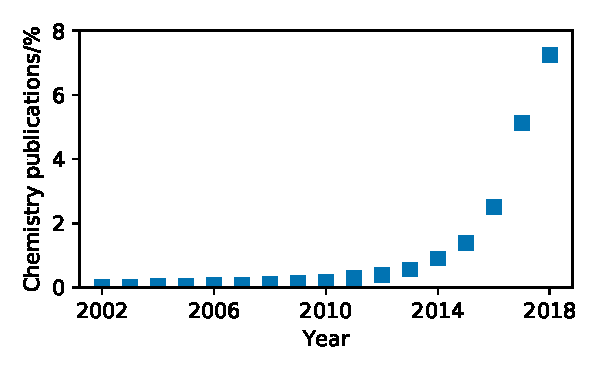
\includegraphics{chem_data_py}
\caption{The percentage of ``chemistry'' publications that mention ``python''. }

Python was first released in 1991, with one of the main design philosophies of the language being code readability. 
This readability is one of the driving factors to its adoption, along with some of the concepts introduced in this course, such as dynamical typing and powerful libraries like NumPy and Matplotlib. 
Since the early 1990s there have been three major versions of Python, with the most recent (and the focus of this course) being Python 3. 
Python 2 is still commonly found online and in libraries, however it is due to ``retire'' at the end of this year (check out https://pythonclock.org for a live countdown). 
Therefore, many packages are now dropping support for Python versions less than 3 and most practitioners would suggest new learners to start with Python 3. 

\section{Variable types}

\bibliographystyle{rsc}
\bibliography{handout_1}

\end{document}